
\chapterauthor{Dinesh Verma}{IBM}
%\chapterauthor{Author Name2}{Affiliation text2}
% \chapterauthor{Author Name3}{Affiliation text3}
% \chapterauthor{Author Name4}{Affiliation text4}

\chapter{AI in the presence of limited connectivity}
\label{chap:limited_network}
%\lipsum[1-2]

This chapter looks at the challenges that arrives when AI/ML based solutions need to be deployed in an environment where the network connectivity is limited. A limited network is one where two communicating parties have limitations on exchanging data with each other. The limitation may arise due to the volume of data being too large compared to the throughput possible on the network, or due to the costs associated with transferring data,  or may be due to regulatory restrictions or security concerns. Regardless of the underlying cause, the basic challenge is that data can not be transferred across the network freely. 

\section{Introduction}
\label{sec:limited_network:intro}
% cover the following topics: 
% Workflow of AI (data collection, train model, inference) 

As mentioned in Chapter~\ref{chap:intro:ai}, an AI enabled system has two distinct stages in its life-cycle. The first stage deals with the creation of an AI model based on training data, and the second stage deals with the use of the AI model to make decisions on an operational piece of data. In both of these stages, limited network connectivity can pose a significant challenge in the effectiveness and operation of a solution. 

During the model creation stage, the key steps include collection of training data, cleaning and curation of the training data, and using the cleaned data to train an appropriate AI model. When the network is constrained, the task of collecting the data can become difficult. 

An alternative to moving the data is to move the training process past the point where the network is limited. However, if data was being collected from different training locations, this means different models trained at different locations need to be combined together. That requires specific mechanisms to handle the limitations. 

During the decision-making stage, operational data has to be used to make decisions. A limited network can make the movement of the operational data to the decision making location difficult. Compounding the challenge is the fact that the devices that may be presented closer to the location where data is being generated may have limited resources. 

\begin{figure}[htbp]
\centering
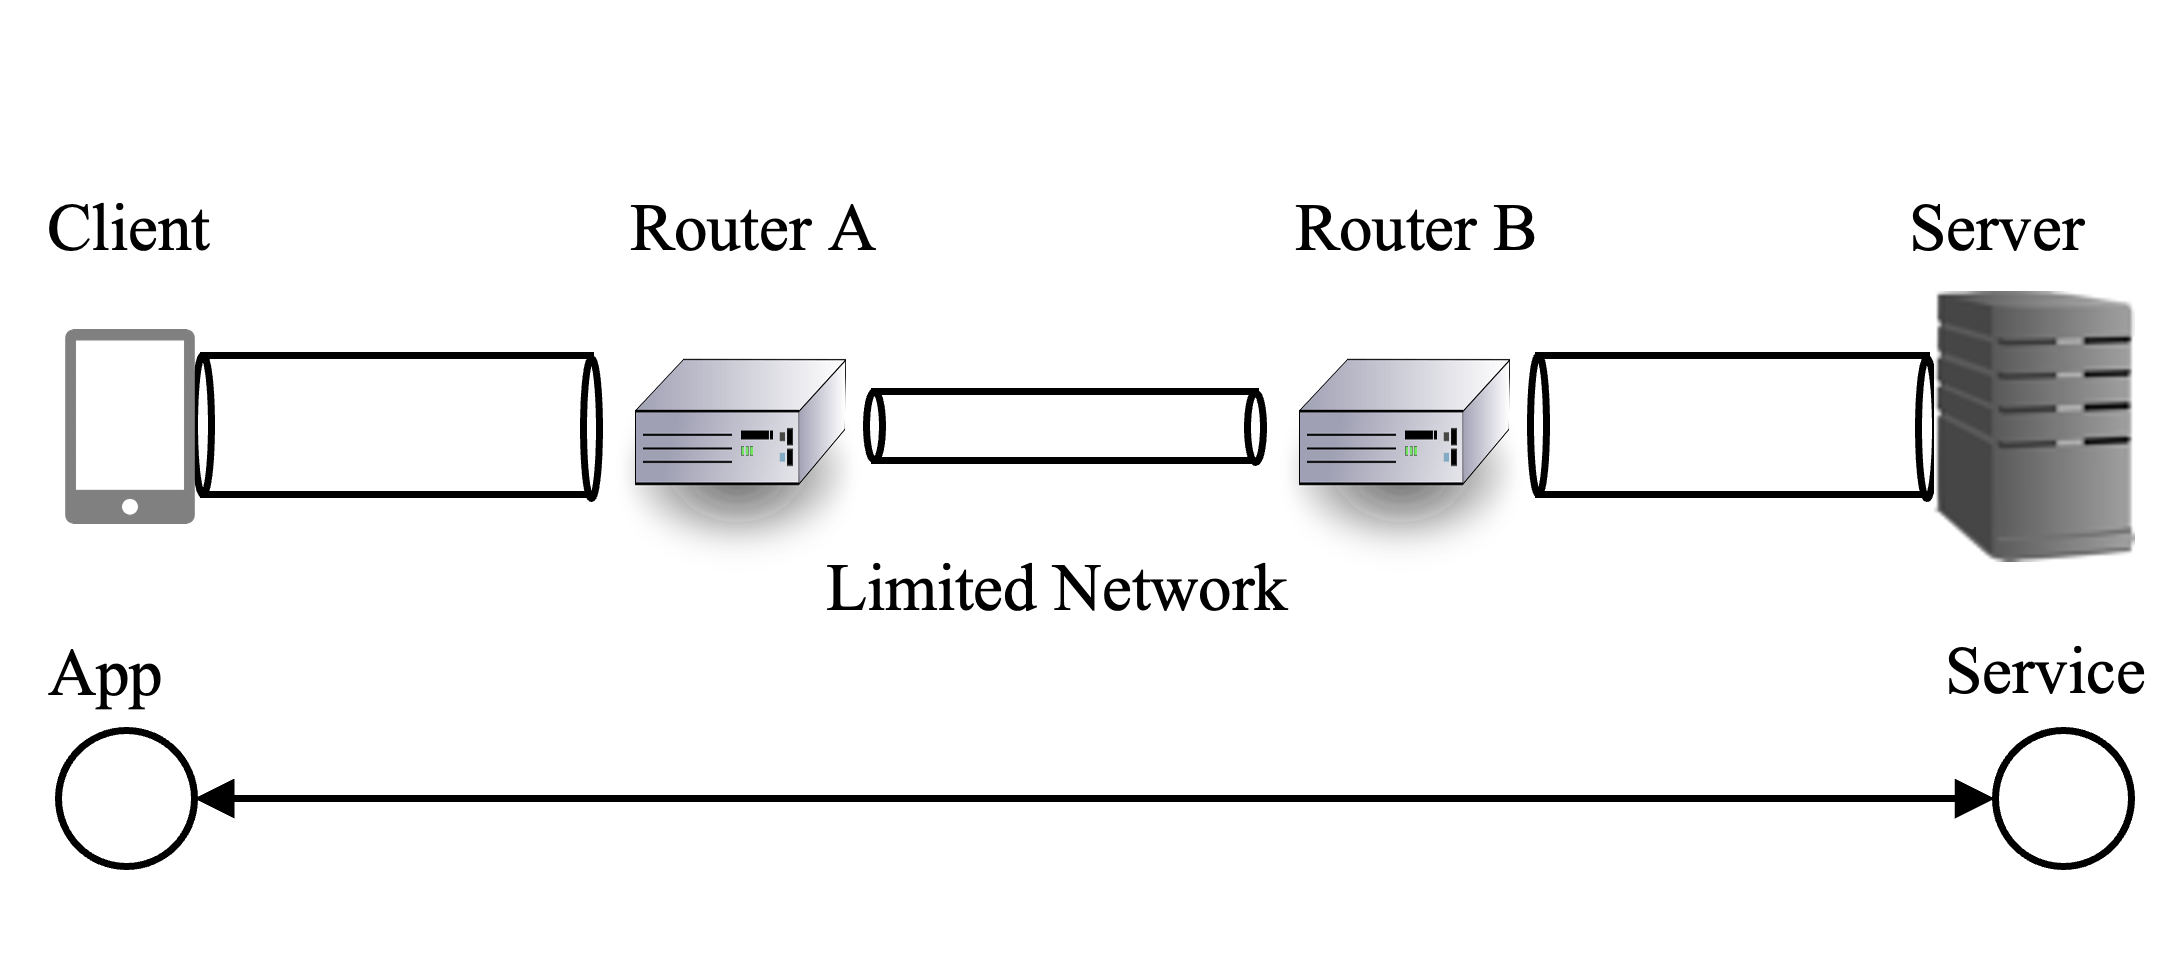
\includegraphics[height=2in] {chapters/chap_net_limited/chap_net_figures/fig1.png}
\caption{Abstracted Model of a Limited Network}
\label{fig:chap_net:ov}
\end{figure}

The challenge of data collection in a limited network environment can be illustrated using the simplified diagram shown in Figure~\ref{fig:chap_net:ov}. This figure shows a simplified model of a limited network. A client accesses a server through a network. Part of the network between the client and the server is constrained. The constrained network is flanked by two routers (A and B) which face the client and the server respectively. The network between the client and the router A and the network between the server and the router B are assumed not to be constrained. 

In these cases, an emerging economy would be on one side of the limited network and the services it wants to access would be on the other side. In other scenarios, the  client and the server may both be within an emerging nation, and the internal network in the nation could be constrained. 

When the application on the client needs to interact with a service on the server, the limited network would have an adverse impact of its performance and responsiveness. 

\section{Data Collection Challenges}
\label{sec:limited_network:collection}

During the task of data collection, we can assume that the client application shown in Figure~\ref{fig:chap_net:ov} is collecting information and sending it to the server shown in the same figure. The client may be a sensor, a microphone, a camera or applications on a phone that use the peripherals or devices within the phone. A phone can in some instances be used to record sounds, upload images and videos. 

The main task of the application on the client is to get the data generated locally successfully uploaded to the service. In order to do that in the presence of the limited network, the application needs to minimize the amount of data that is transferred over the constrained network. One approach to do such minimization is to compress the data flowing between the client and the server. 

This process is shown in Figure~\ref{fig:chap_net:compress}. A compression and a decompression function are introduced between the client and the server. The information from the client is compressed before it is sent over the limited network, and it is uncompressed after it leaves the limited network. 

The location of the compression function can be anywhere from the application (on the client device) to any (and including) device upto router A. Similarly, the location of the uncompression function can be anywhere between the server and router B. Since the networks between these segments are assumed to be fast without any constraints, the location would not have a material impact on the performance. 

When data is sent from the server to the client in the reverse direction, the tasks of compression and decompression needs to be performed in reverse location. However, since we are assuming that the data is primarily flowing from the client to the server, the compression is shown on the client side while the decompression is shown in the server side. In many sites, the site for compression and decompression would perform these operations for data flowing in both directions. 

\begin{figure}[htbp]
\centering
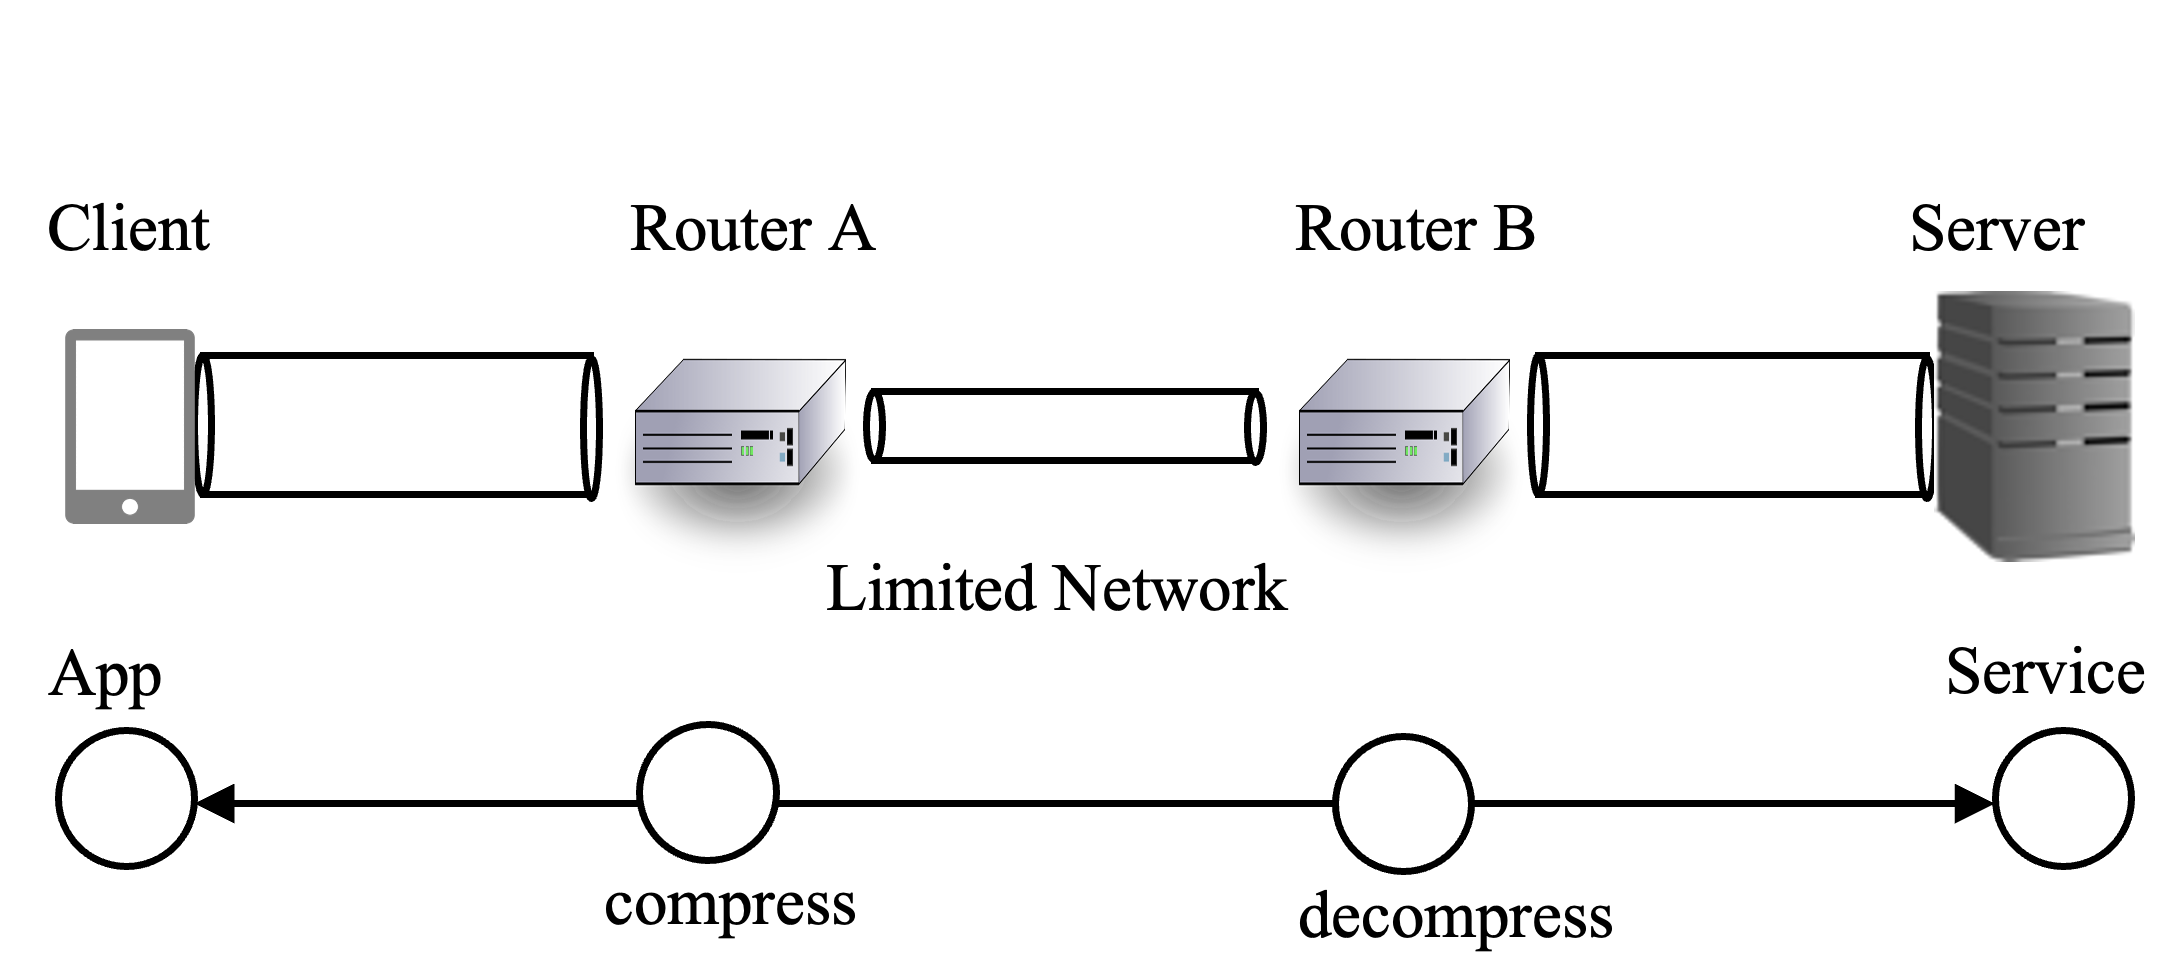
\includegraphics[height=2in] {chapters/chap_net_limited/chap_net_figures/fig2.png}
\caption{Compression to reduce data transfer}
\label{fig:chap_net:compress}
\end{figure}

There are many types of compression algorithms that can be used to reduce the amount of information flowing through a constrained network link.  Compression algorithms are classified into the two broad categories of lossless compression and lossy compression. In lossless compression, data is compressed so that the entire original data object can be reconstructed without any errors. In lossy compression, portions of the original data object are considered less important, and a better reduction is obtained by using approaches where those portions are discarded. Lossless compression is used for general data objects, while lossy compression is used for objects where some amount of loss can be tolerated, e.g. audio or video content where humans are able to make sense even if the content is slightly degraded. 

A commonly used set of lossless compression algorithms belong to the Lempel-Ziv family ~\cite{ziv1977universal, ziv1978compression}. These algorithms look for repeated patterns or sequences occurring in the content, and replace them with equivalent smaller representations on subsequent occurrences. The algorithm creates a table to store bit-patterns against the shorter representations. The table is generated dynamically depending on the contents of the object being compressed.

Lossy compression is usually more efficient than lossless compression. Some common standards, e.g. JPEG, MPEG and MP3 for audio/video use variations of lossy compression. In these schemes, the algorithm drop portions of the  data that is less important. See ~\cite{david2004data, sayood2017introduction} for a survey of both lossy and lossless data compression algorithms. 

One type of compression scheme is called byte-caching~\cite{le2012byte}, in which a dictionary is maintained between two devices with frequently occurring content replaced with a small  hash. Byte-cache builds the dictionary dynamically based on the contents of the packets  flowing between two pair of devices. The bytes that are to be matched with specific hash-codes are maintained in a cache at each of the devices, hence the name byte-cache. 

Byte caching relies on a shared dictionary to reduce size of data flowing between two devices. Other variations on dictionary based payload compression include maintaining multiple dictionaries at each point and selecting them on a packet by packet basis based on the content, or creating estimates for predicting future byte-streams based on current content, which may allow for more efficiency

If the network link is very constrained, e.g. a satellite link, one can deploy header compression~\cite{tye2003review} which tries to minimize the overhead in transmission of information. Standard headers protocols used for communication (e.g. in the Internet family of TCP/IP protocols) are designed for a general purpose network, and some of their fields may not be very useful under some special situations. Standards to compress headers are part of communication standards ~\cite{rfc1144, rfc2507, rfc3544}. Many of the fields in the packet header do not change frequently on some links. As an example, if a source and destination are communicating on a serial link, these two fields are going to remain the same regardless of the packet exchange. In these cases, one can use a streamlined header that does not require specifying these fields.

Some objects being transferred on the mobile network can be made available in different formats, with each format using a different amount of bandwidth on the network. Video streams, for example, can be encoded at different rates~\cite{pancha1994mpeg}. Many common types of video encoding schemes ~\cite{li2001overview} produce video that contains a base layer and several enhancement layers. The video quality is acceptable when only the base layer is sent to the receiver and becomes better as more and more enhancement layers are used. This allows a sender to control the data that a video stream consumes depending on the rate that is available.  


\begin{figure}[htbp]
\centering
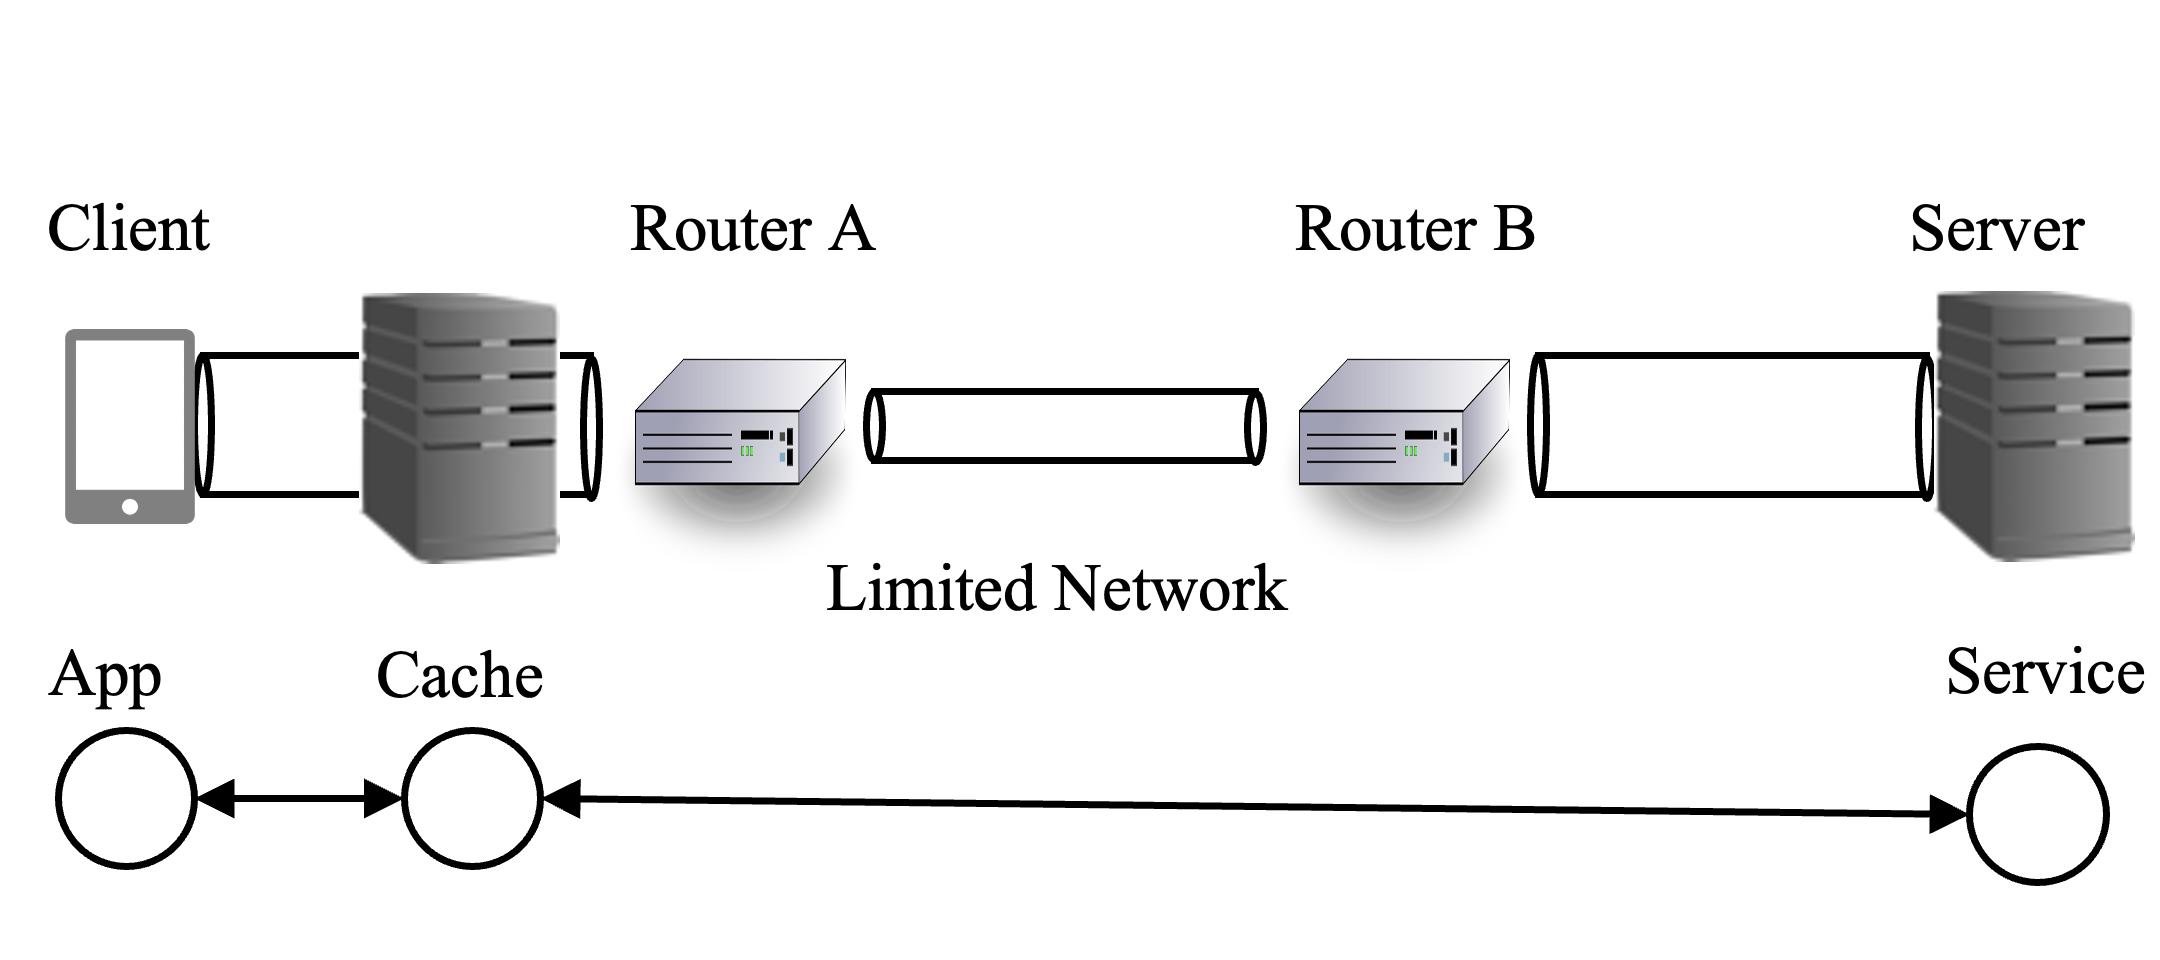
\includegraphics[height=2in] {chapters/chap_net_limited/chap_net_figures/fig3.png}
\caption{Caching to bypass data collection in a Limited Network}
\label{fig:chap_net:cache}
\end{figure}

In some cases, there may be many applications that may need to collect the same data source. For example, let us consider an emerging economy where several researchers are interested in training a machine learning model to understand the satellite imagery. In order to train the imagery, they can use imagery data that is available from various government agencies in US and Europe. If there are multiple users of the same data, it is possible to set up a caching service for the data in the nation itself. The caching service can retrieve the data once, and then let the other users obtain the data from the cache instead of obtaining it from the service across the constrained network. This setup is shown in Figure~\ref{fig:chap_net:cache}. 

While the caching approach works well in a technical sense, there may be some business issues which are hard to work around. If the different developers in the emerging economy belong to different companies, who should be the company running and operating the caching service? Is it appropriate for the caching service to redistribute content that belongs to some other entity -- one that holds the original data? The incentives to deploy a caching solution to reduce the bandwidth passed on the constrained link may not always be clear.   

Since we know the the data collection is meant for machine learning purposes, there are some other compression techniques that can also be used that are specific to machine learning. One such approach is the use of core-sets ~\cite{ mirzasoleiman2020coresets, lu2020robust}. When machine learning training data is collected, some of the training data may be redundant for the machine learning algorithm, in the same that it does not provide any additional new information that improves the model. The goal behind core-sets is to reduce the amount of data so that the quality of machine learning model is not compromised, but data points that do not improve the model are ignored. This provides an application-specific approach to compression. 

Another approach for reducing data compression is to only select data relevant for the machine learning task. As an example, suppose a data source is available on a well-connected portion of the Internet, e.g. satellite images may be available from the U.S. or European government agencies. A developer in an emerging economy wants to use those data sets to train machine learning models. The developer and the data source are separated by a trans-oceanic network which is expensive, high-latency and high-delay. It is worthwhile to note that all the data available in the US/European agency would not be relevant to the task of building a machine learning model in the emerging nation. As an example, the image data may cover all of the world, but the developer may want to train a model on the data collected for one country only. The developer could choose to use a computer located in US/Europe to download the whole data set, select the relevant parts of data of interest to the machine learning task, and only take that subset of data across the constrained link. This can cut down on the amount of data being transferred. 

\section{Model Training with limited networks}
\label{sec:limited_network:training}

% Moving model training to the edge (linear topology)
% data curation/labeling challenges
% federated learning (model iteration) 
% One-Shot federated learning 

\begin{figure}[htbp]
\centering
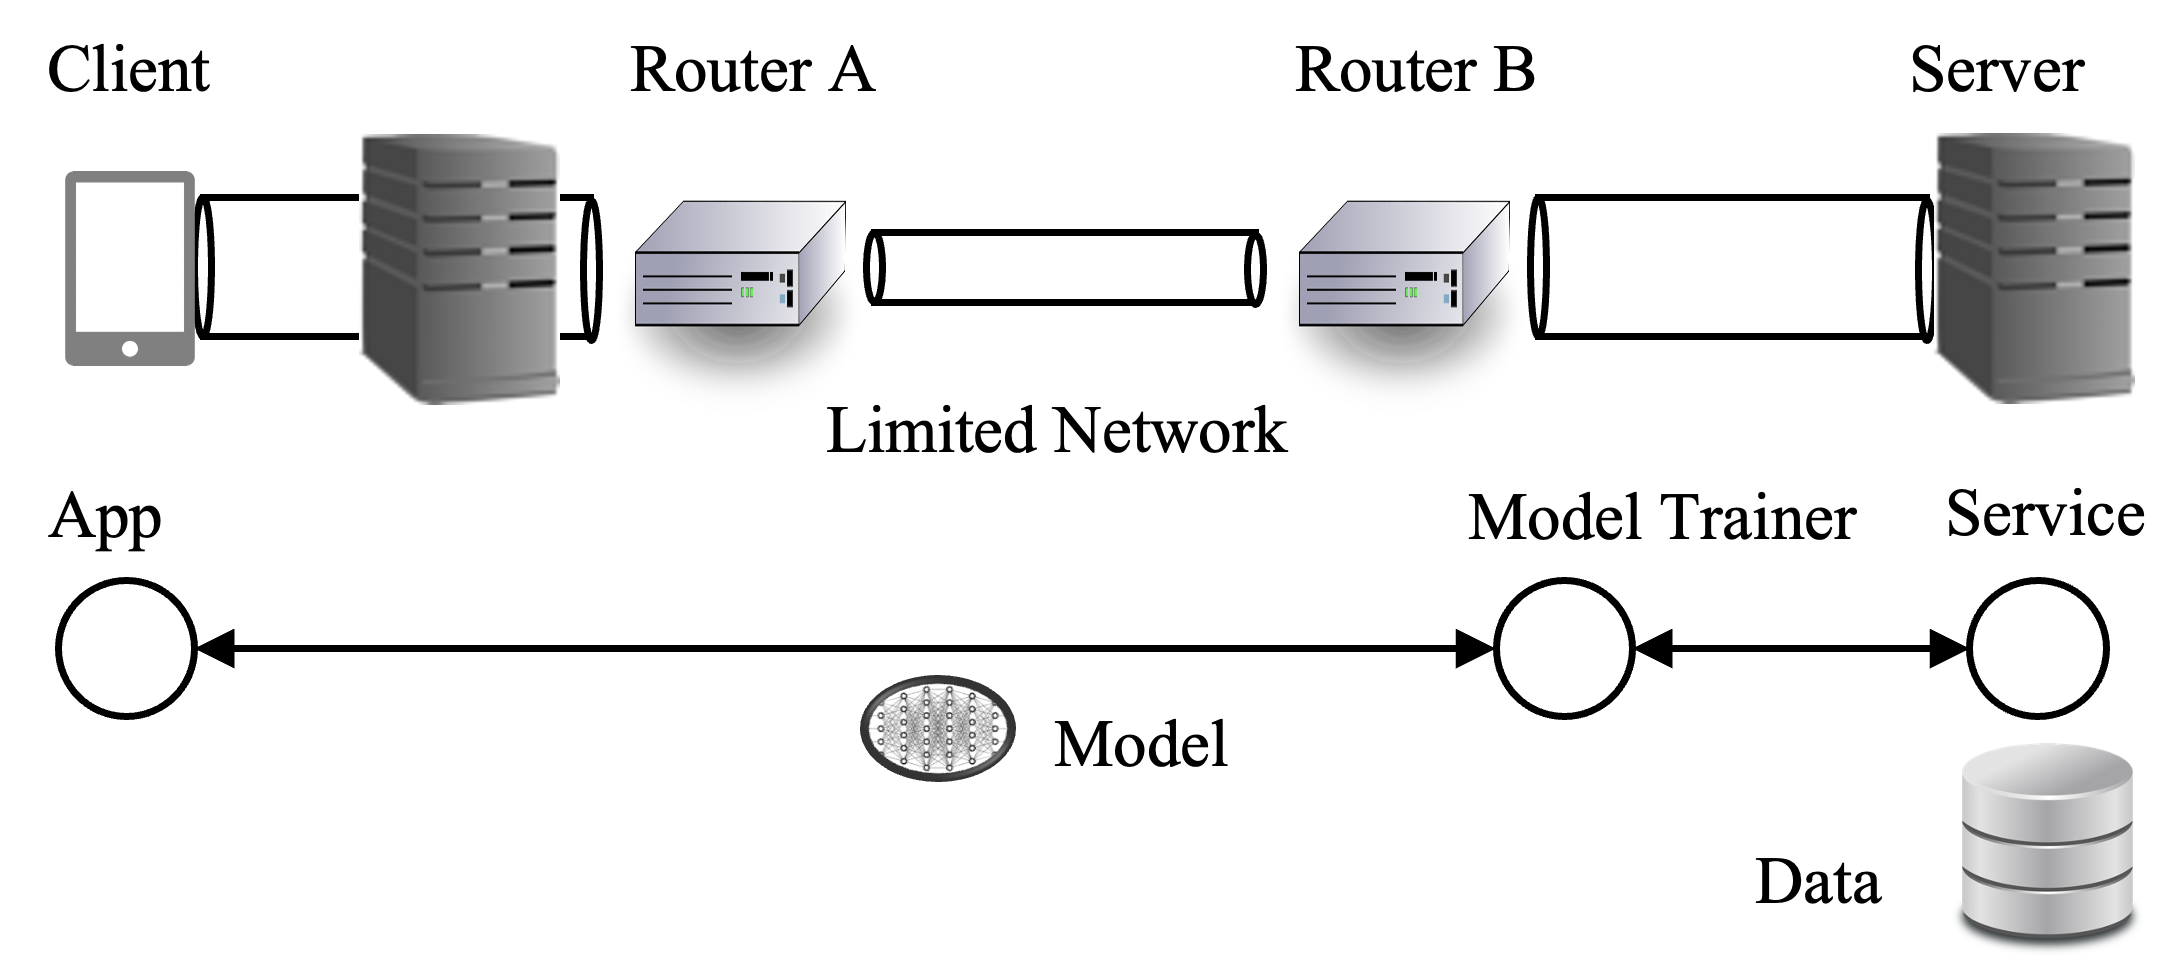
\includegraphics[height=2in] {chapters/chap_net_limited/chap_net_figures/fig4.png}
\caption{Learning past the Constrained Link}
\label{fig:chap_net:edge_learn}
\end{figure}


When model training needs to be done on a data source which is across a constrained network, another approach would be to avoid the constrained link altogether for data movement. If the model training process is moved over to the other side of the constrained link, one can only move the model across the constrained link. In general the model would be significantly smaller than the amount of data used to train it. 

This approach is shown in Figure~\ref{fig:chap_net:edge_learn}. Suppose data is present on the right-hand side of the system. Even though the client needing the data is present on the left-hand side, it is better to train an AI model on the right-hand side, and move the model instead of moving the data across the link. 

\begin{figure}[htbp]
\centering
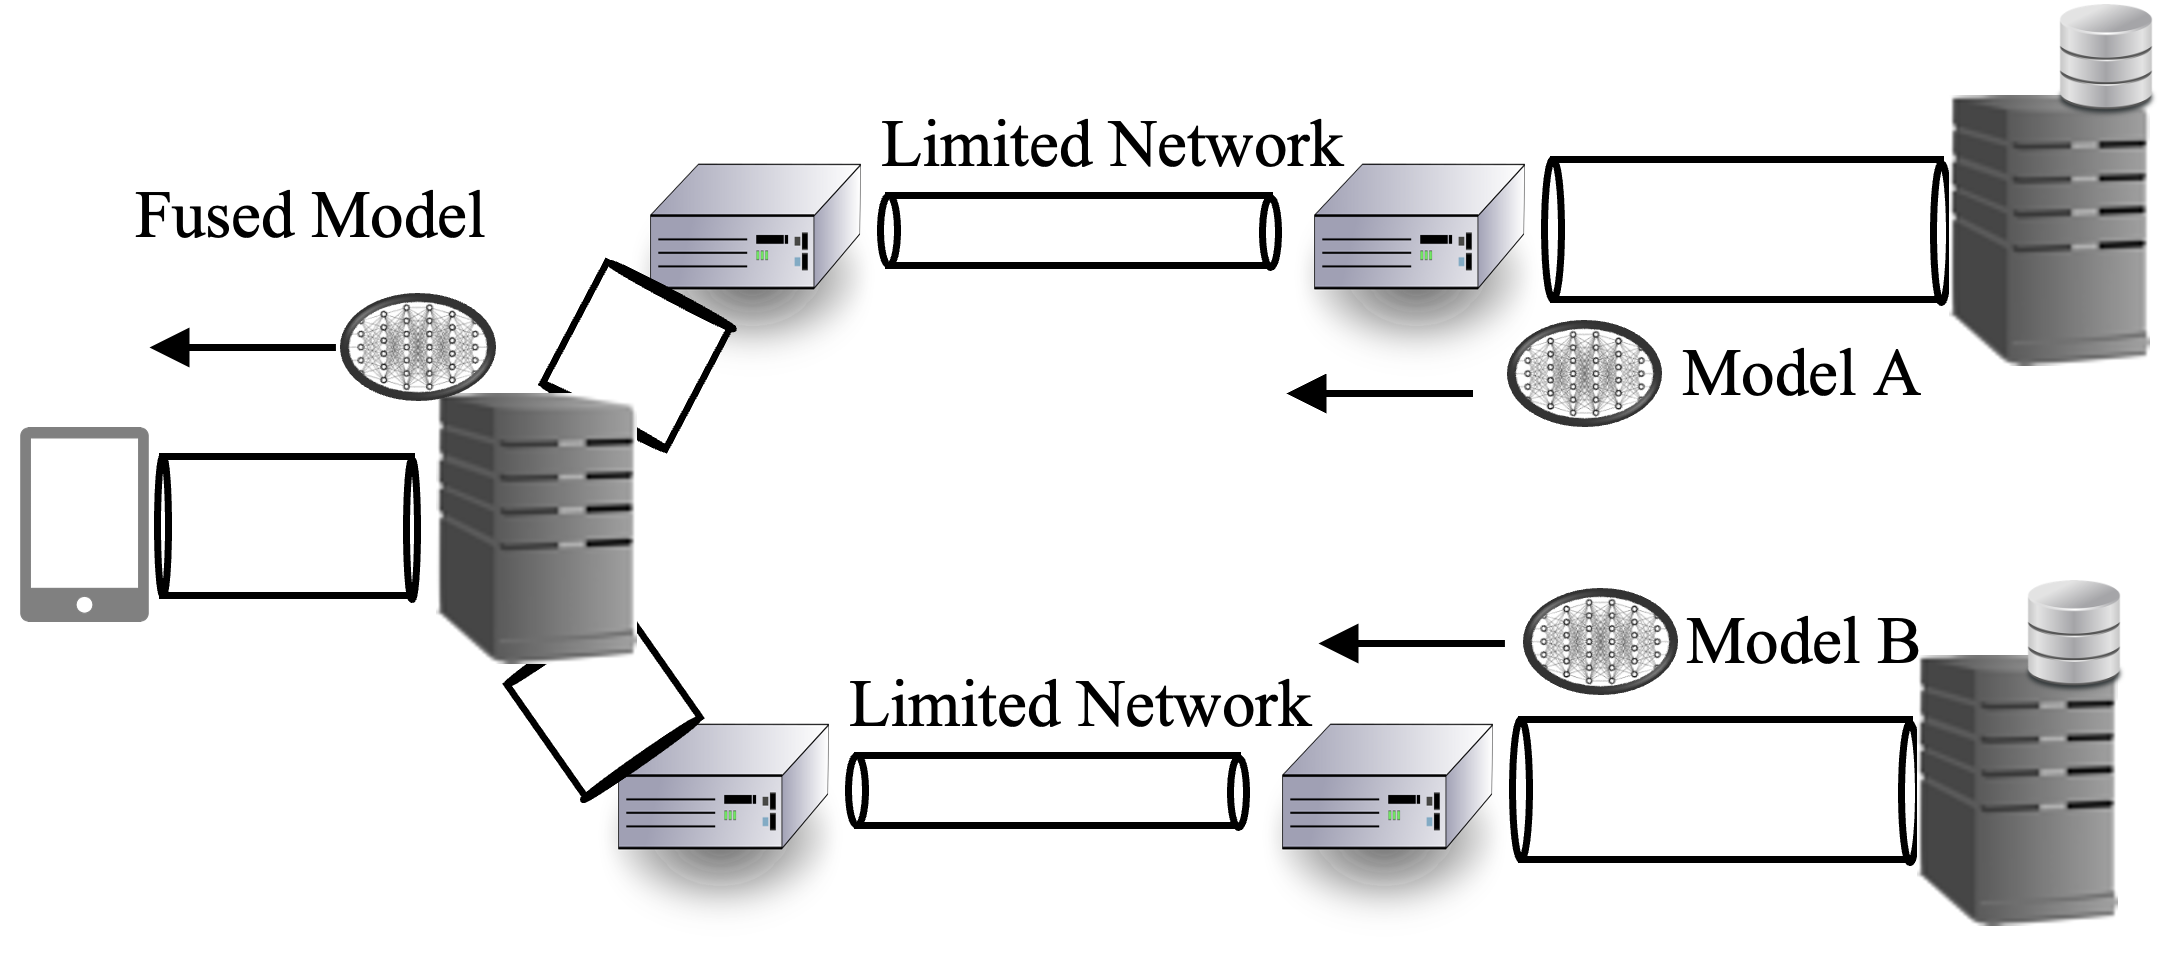
\includegraphics[height=2in] {chapters/chap_net_limited/chap_net_figures/fig5.png}
\caption{Federated Learning with a Limited Network}
\label{fig:chap_net:fedlearn}
\end{figure}

In some cases, the data may not be present at a single location but at many different locations. In some cases, the constraints on the data may be on accessing the different data sources. As an example, consider the situation of three different emerging nations, all of whom have data related to agricultural crops in their nations respectively. Ideally, they want to combine the data together. However, moving the data across the links may be too time-consuming. 

The techniques for federated learning~\cite{verma2021federated}
may be useful here. In Federated learning, each of the emerging nations can train their own models independently, and then the models are combined together into an aggregated combined model. Since the approach moves models over the constrained link, it works better than moving the data across. In using federated learning, an approach that minimizes the movement of models across the constrained links ~\cite{verma2022non} works better than those that move models multiple times. 

A sample scenario for federated learning is shown in Figure~\ref{fig:chap_net:fedlearn}. The figure takes the hypothetical situation where training data is present in two different locations, and each location has a limited network to the place where the model resulting from the training of the data is used, namely the client. The approach would be to have another server which is used to combine models trained by each of the locations with data. This setup can be useful for countries to share models with each other instead of sharing raw data with each other. 


\section{Inference with limited networks}
\label{sec:limited_network:inference}

% Three approaches 
% Compress data -- e.g. PCA or some other reduce representation 
% Move inference across the edge past the low latency 
% Move some layers to the edge, other layers at original site. 

% Make reference to the fact that optimization needs to be handled in the different stages. 
% Limited model - model optimization (chapter 2.2)



